
%
\begin{figure}[t]
	\centering
	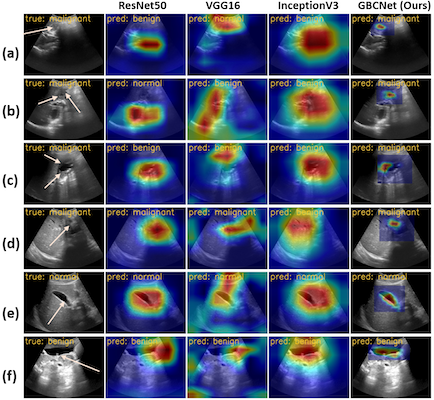
\includegraphics[width=0.62\linewidth]{figs/gbcnet/grad-cam.png}
	\caption[Qaualitative analysis of GBCNet with Grad-CAM visuals]{Grad-CAM visuals and the predictions for ResNet50, VGG16, Inception-V3, and GBCNet. The pathological areas are shown with arrows in the original images. 
	(a) ResNet50 and Inception-V3 focus on the shadow, whereas VGG16 focuses on the echogenic area, and all three fail to detect \gbc. GBCNet accurately focuses on the malignant \gb region invading the liver and detects \gbc.  (b), (c) The baseline networks focus on shadow or noise instead of the cancerous area and mispredict. 
	(d) Although ResNet50 and VGG16 predict malignancy, they fail to precisely focus on the malignant region compared to GBCNet. Inception-V3 failed to classify \gbc. (e), (f) GBCNet pinpoints the discriminating region compared to the baselines for normal and benign \gb regions, respectively. More visuals provided in \cref{fig:supple-2}.} %\ref{supp:cam_vis}.}
	\label{fig:gbc_vis}
\end{figure}

\begin{figure}[t]
	\centering
	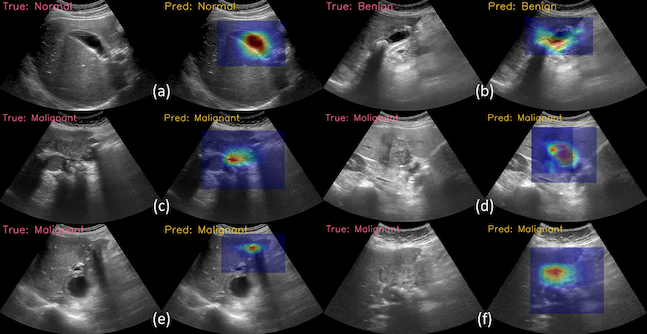
\includegraphics[width=0.7\linewidth]{figs/gbcnet/vis-s-1.png}
	\caption[Additional Grad-CAM visuals for GBCNet]{Sample Grad-CAM visuals of GBCNet with curriculum learning. (a) Normal, (b) Benign, and (c)--(f) Malignant samples.}
	\label{fig:supple-2}
\end{figure}

\section{Experiments and Results}
%
\subsection{Dataset}
%
We have used the image-based GBCU dataset described in \cref{chap:data} for the experiments. We recall that, there is a total of 1255 B-mode static abdominal USG images collected from 218 patients in this dataset. Each image is labeled as one of the three classes - normal, benign, or malignant, based on the biopsy reports. In addition to the classification labels, each image contains an axis-aligned bounding box spanning the entire \gb and adjacent liver parenchyma to annotate the \roi. The \roi in each image is drawn in consensus by two expert radiologists with 10 and 2 years of experience in abdominal radiology. The \roi (bounding box) annotations were used to train the \gb region selection network in the first stage of the GBCNet. The classification network in the second stage was trained using the image class labels. 

\mypara{Dataset Statistics}
%
Overall, we have 990 non-malignant (432 normal and 558 benign) and 265 malignant images. Of the 218 patients, 71, 100, and 47 belong to the normal, benign, and malignant classes, respectively. The width of the images was between 801 to 1556 pixels, and the height was between 564 to 947 pixels due to the cropping of patient-related information. 

\mypara{Dataset Splits}
%
The sizes of the training and testing sets are 1133 and 122, respectively. To ensure generalization to unseen patients, all images of any particular patient were either in the train or the test split. The number of normal, benign, and malignant samples in the train and test set is 401, 509, 223, and 31, 49, and 42, respectively. 
Since the dataset size is small, we also report the 10-fold cross-validation metrics on the entire dataset for key experiments to assess generalization. All images of any particular patient appeared either in the training or the validation split during the cross-validation. 

\subsection{Efficacy of GBCNet over Baselines}
%
We compare GBCNet with three popular deep classifiers, ResNet-50 \cite{resnet}, VGG-16 \cite{vgg}, and Inception-V3 \cite{inception}. We also evaluate the performance of three \sota object detectors, Faster-RCNN \cite{fasterrcnn}, RetinaNet \cite{retinanet}, and EfficientDet \cite{efficientdet} for detecting \gbc. We report the results in \cref{tbl:perf_gbc}. From the reported results, it is clear that baseline networks have poor accuracy for detecting \gbc from \usg images. Grad-CAM \cite{gradcam} visualizations in \cref{fig:gbc_vis} show that the noise, textures, and artifacts significantly influence the decision of baseline classification models. Additionally, \cref{fig:supple-2} shows the sample Grad-CAM visualizations of the predictions using GBCNet (ROI+MS-SoP) with curriculum learning. As highlighted in \cref{sec:usg_artifact_issue}, the standard DNN models tend to focus on the large shadow regions, and as a result, their classification accuracy suffers heavily. The shadow regions resembles the visual characteristics of a normal gallbladder (dark, anoechoic region). Compared to the baselines, GBCNet along-with the proposed MS-SoP classifier precisely focuses on crucial visual cues leading to its superior performance. 
%
\begin{table}[t]
	\centering
	\footnotesize
%	\captionsetup{width=\linewidth}
%    \setlength{\tabcolsep}{6pt}
%	\resizebox{\linewidth}{!}
	\caption[Comparison of the \gb region selection models]{Comparison of the \gb region selection models. We reported 10-fold cross validation (Mean$\pm$SD) of the metrics.}
\label{tbl:perf_region}
\end{table}
%
\begin{figure}[t]
	\centering
	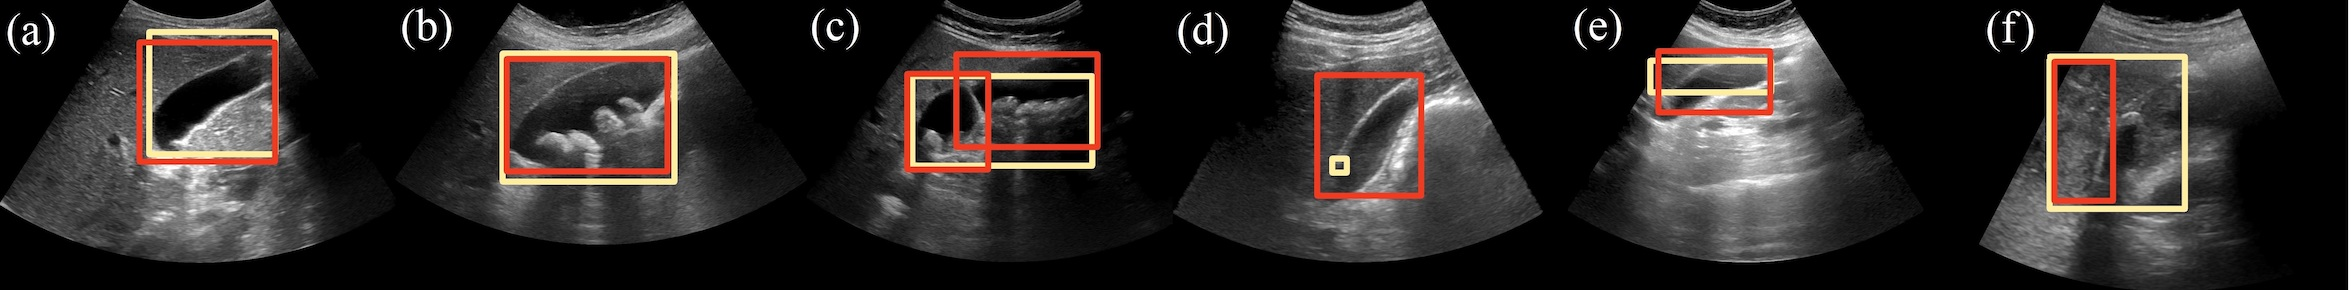
\includegraphics[width = \linewidth]{figs/roi_preds.jpg}%{figs/gbcnet/roi_preds.jpg}
	\caption[Comparison between the ROIs predicted by Faster-RCNN with radiologists]{We visually compare \roi selection by Faster-RCNN (dark red) with the \roi identified by expert Radiologists (light yellow). (a, b) The predicted a\roi matches well with the radiologists' expectations. (c) The model considers the sections partitioned by the \gb wall as separate regions. However, the union of the predicted boxes very closely approximates the actual \gb region. (d, e) Although the radiologist made an error in judging the \roi, Faster-RCNN was able to identify an accurate \roi resulting in a visually superior prediction. (f) The predicted \roi covers only a portion of the area an expert radiologist considered necessary. Even though the region prediction seems inferior compared to the human perception, expert radiologists corroborated that the predicted region captures the \gb invading the liver, a vital visual cue to detect \gbc. \roi samples from other detectors are in Appendix \cref{fig:supple-1}.}
	%\ref{supp:roi_vis}.}
	\label{fig:region_vis}
\end{figure}
%
\begin{figure}[t]
	\centering
	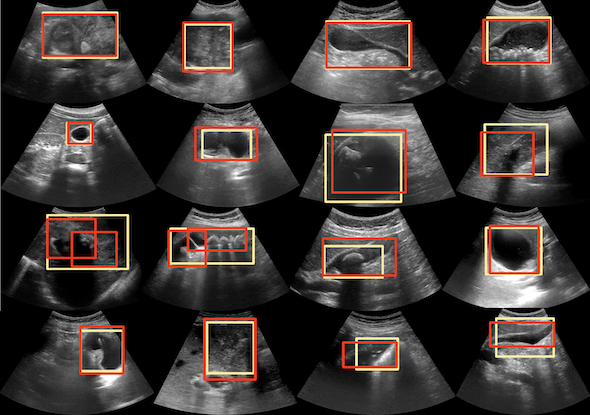
\includegraphics[width=0.7\linewidth]{figs/gbcnet/vis-s-0.png}
	\caption[Additional ROI visuals]{Sample visual results of RoI Detection models. First row - Faster-CNN, second row - YOLOv4, third row - Reppoints, and fourth row - CentripetalNet. Dark red is the ROI prediction by the model and light yellow is expert radiologists' perception of ROI.}
	\label{fig:supple-1}
\end{figure}
%
%\section{Appendix}
%
%
%\subsection{GradCAM Visuals for GBCNet}
%\label{supp:cam_vis}
Figure \ref{fig:supple-2} shows the sample Grad-CAM visualizations of the predictions using GBCNet (ROI+MS-SoP) with curriculum learning. %The blue regions show the most vital regions used by the classifier during prediction. The classifier well emphasized the crucial visual cues during inference.  

% \subsection{Candidate ROI Visuals}
% \label{supp:roi_vis}
% In figure \ref{fig:supple-1}, we show sample predictions of the GB region localization for different models. We also show the region of interest as perceived by the expert radiologists. The localization model is fairly accurate in capturing important regions of the USG image.

%
%
%\mypara{Performance of \gb Region Selection Models}
\subsection{Performance of GB Region Selection Models}
%
\cref{tbl:perf_region} summarizes the performance of various models for localizing the \gb region. For critical tasks such as region selection for cancer detection, recall is more important than precision. Multiple predicted regions can be discarded in the second stage, but missing any potentially malignant region could be disastrous. We note that the Faster-RCNN achieves the highest mIoU out of all the models while maintaining very high recall and excellent precision. Hence, we use Faster-RCNN as the region selection model. In \cref{fig:region_vis} we show the visual comparison of the \gb localization results of Faster-RCNN along with the \rois annotated by the expert radiologists. The model could predict the region of interest accurately in most cases. Although the model's prediction visually differed from the radiologists in some samples, closer inspection revealed that the predicted region retains sufficient visual cues to detect malignancy. In figure \ref{fig:supple-1}, we show additional sample predictions of the GB region localization for different models. 

\begin{table}[t]
	\centering
    \footnotesize
    \begin{tabular}{@{}lccc@{}}
    \toprule[1pt]
    \textbf{Model} & \textbf{Spec.} & \textbf{Sens.} \\
    \midrule[0.5pt]
    ResNet50 &  0.975 $\pm$ 0.024 & 0.829 $\pm$ 0.088\\
    DenseNet121  & 0.968 $\pm$ 0.018 & 0.824 $\pm$ 0.027 \\
    \midrule[0.5pt]
    MS-SoP (ours) & 0.967 $\pm$ 0.027 & 0.871 $\pm$ 0.071 \\
    \bottomrule[1pt]
    \end{tabular}
	\caption[Breast cancer detection results]{The sensitivity and specificity of MS-SoP and two baseline classifiers on breast cancer detection from USG images. We report 5-fold cross-validation on the BUSI dataset.}
\label{tbl:busi}
\end{table}

\begin{table}[t]
	\centering
	\footnotesize
	%\captionsetup{width=\linewidth}
    %\setlength{\tabcolsep}{10pt}
%    \resizebox{ \linewidth}{!}{%
    \begin{tabular}{lcccc}
    \toprule[1pt]
    \multirow{2}{*}{\textbf{Model}} & \multicolumn{2}{c}{\textbf{Orig. Test Set}} & \multicolumn{2}{c}{\textbf{Synth. Test Set}} \\
    & \textbf{Spec.} & \textbf{Sens.} & \textbf{Spec.} & \textbf{Sens.}\\
    \midrule[0.5pt]
    %AR+VGG16 & 51.6 & 56.3 & 88.1 & 55.7 ($\downarrow$) & 62.5 ($\downarrow$) & 88.1 \\
    ROI+VGG16 & 0.838 & 0.572 & 0.787 ($\downarrow$~~6.1\%) & 0.572 \\
    ROI+VGG16+VA & 0.825 & 0.762 & 0.775 ($\downarrow$~~6.1\%) & 0.762 \\
    \midrule
    %AR+ResNet50 & 84.3 & 85.7 & 88.6 & 71.3 ($\downarrow$) & 65.0 ($\downarrow$) & 88.6 \\
    %AR+ResNet50+curriculum & 91.8 & 93.8 & 97.6  & 88.5 ($\downarrow$) & 87.5 ($\downarrow$) & 97.6 \\
    ROI+ResNet50 & 0.863 & 0.857 & 0.650 ($\downarrow$24.7\%)& 0.857 \\
    ROI+ResNet50+VA & 0.938 & 0.857 & 0.887 ($\downarrow$~~5.4\%) & 0.857 \\
    \midrule
    ROI+Inception-V3 & 0.563 & 0.833 & 0.413 ($\downarrow$26.6\%) & 0.833 \\
    ROI+Inception-V3+VA & 0.913 & 0.690 & 0.788 ($\downarrow$13.7\%) & 0.690 \\
    \midrule
    GBCNet & 0.900 & 0.929 & 0.762 ($\downarrow$15.3\%) & 0.929 \\
    GBCNet+VA & 0.950 & 0.976 & 0.850 ($\downarrow$10.5\%) & 0.976 \\
    \bottomrule[1pt]
    \end{tabular}
%    }
    \caption[Robustness of the visual acuity curriculum in tacking texture bias]{Robustness of the curriculum in tacking texture bias while detecting \gbc. We show the performance of using curriculum on four models that apply classifiers on localized \gb region - (a) ROI+VGG16, (b) ROI+ResNet50, (c) ROI+Inception-V3, and (d) GBCNet (ROI+MS-SoP). The relative change (in percentage) in specificity for synthetic test data is shown within parentheses. The sensitivity remains unchanged as the malignant images were not altered. Observe that as compared to the models trained on high-resolution images, our VA-based curriculum is more robust to textures and is able to maintain a lower drop in specificity. The only exception is the ROI+VGG16 model, for which the curriculum training does not lower the drop in specificity. }
    %Also, note how the proposed curriculum is able to improve the performance of all four networks.}
\label{tbl:curr_texture}
\end{table}

\subsection{Applicability of the Proposed Classifier in Breast Cancer Detection from USG Images}
%
We explored the applicability of the proposed MS-SoP classifier on breast cancer detection from \usg images for a publicly available dataset, BUSI \cite{al2020dataset}, containing 133 normal, 487 benign, and 210 malignant images. The images in BUSI are already cropped from original \usg images to highlight only the important regions. Thus, we skip the \roi selection and run the MS-SoP classifier on BUSI. \cref{tbl:busi} shows that the MS-SoP classifier achieves much better sensitivity, which indicates the superiority of the MS-SoP architecture for malignancy identification on \usg images. We note that while breast cancer detection relies on tissue/ mass characterization, \gbc detection is primarily based on wall shape and mass anomaly. %The performance gain using MS-SoP on these two different types of cancers is interesting to note.
\par We remark that, while the MS-SoP classification network was applicable on both tasks, the Visual Acuity-based curriculum may not be suitable for Breast Cancer Detection. Breast cancer detection from USG relies heavily on the textures of the mass/ tissue in the images, as opposed to the wall shape and mass forming anomalies in GBC. Thus, while using a smoothing-based curriculum to bias the learning towards shape features is conducive for GBC detection, it may not aid breast cancer detection.

\begin{figure}[t]
	\centering
	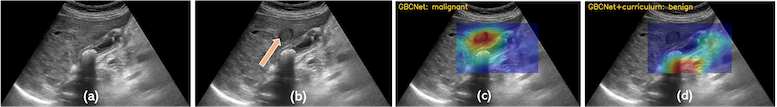
\includegraphics[width=0.9\linewidth]{figs/gbcnet/texture_vis_curr.png}
	\caption[Visualization of the effect of curriculum]{(a) Original image of a benign \gb. The \gb presents a stone and thickened wall. (b) In the synthetic image, we added an artificial tissue-like patch near the benign \gb region (highlighted by the arrow). This patch is not a part of the original \gb, and expert radiologists confirmed that the diagnosis of the \gb is not altered. (c) The textured artificial patch makes the GBCNet biased, and it focuses on the patch to predict the sample as malignant (false-positive). (d) Visual acuity curriculum fixes the texture bias of the GBCNet and helps the network to re-adjust the salient regions to the actual \gb pathology. %and learn the visual cues of a non-malignant \gb such as stone or a thickened wall.
}
	\label{fig:texture_vis}
\end{figure}

\subsection{Efficacy of the Proposed Curriculum}
%
\myfirstpara{Robustness in Tackling Texture Bias}
As described earlier, spurious textures present in \usg images tend to increase the false positives in detecting malignancy. To validate this hypothesis, we created a synthetic test set. We used the method given by \cite{yang2020fda} and added low-level frequencies from malignant images to alter the original texture of normal and benign samples. We also manually added patches looking like soft tissue near the \gb region of normal and benign images. Expert radiologists confirmed that the diagnosis of the \gb pathology is not altered. \cref{tbl:curr_texture} shows that the specificity decreases due to the increase of the false positives. The sensitivity remains unaffected as the prediction for malignant \gb samples was unchanged. The network trained with the proposed curriculum tackles texture bias well and accurately predicts non-malignant samples in synthetic test data. This experiment shows that the proposed curriculum effectively tackles texture bias. \cref{fig:texture_vis} shows a visual sample of how the soft tissue-like texture influences the network's decision and how the curriculum helps the network to rectify the discriminative regions. 

\begin{table}[t]
	\centering
	\footnotesize
%	\captionsetup{width=\linewidth}
%    \setlength{\tabcolsep}{6pt}
%	\resizebox{\linewidth}{!}{%
    \begin{tabular}{@{}lccc@{}}
    \toprule[1pt]
    \textbf{Model} & \textbf{Acc} & \textbf{Spec.} & \textbf{Sens.} \\
    \midrule[0.5pt]
    ROI+VGG16 & 0.533 $\pm$ 0.092 & 0.719 $\pm$ 0.115 & 0.733 $\pm$ 0.179\\
    ROI+VGG16+VA & 0.777 $\pm$ 0.041 & 0.938 $\pm$ 0.030 & 72.0 $\pm$ 0.195\\
    \midrule
    ROI+ResNet50 & 0.766 $\pm$ 0.107 &  0.823 $\pm$ 0.105 & 0.909 $\pm$ 0.111\\
    ROI+ResNet50+VA & 0.854 $\pm$ 0.077 & 0.923 $\pm$ 0.059 & 0.875 $\pm$ 0.091 \\
    \midrule
    ROI+Inception-V3 & 0.718 $\pm$ 0.089 & 0.833 $\pm$ 0.087 & 0.785 $\pm$ 0.214\\
    ROI+Inception-V3+VA & 0.826 $\pm$ 0.046 & 0.931 $\pm$ 0.044 & 0.826 $\pm$ 0.099\\
    \midrule
    % RetinaNet & 74.9 $\pm$ 7.3 &  86.7 $\pm$ 7.8 & 79.1 $\pm$ 8.9\\
    % RetinaNet+VA & 73.3 $\pm$ 6.0 & 92.1 $\pm$ 4.4 & 70.6 $\pm$ 14.2\\
    % \midrule
    GBCNet (ROI+MS-SoP) & 0.882 $\pm$ 0.051 & 0.942 $\pm$ 0.037 & 0.923 $\pm$ 0.071\\
    GBCNet+VA & 0.921 $\pm$ 0.029 &  0.967 $\pm$ 0.023 & 0.919 $\pm$ 0.063\\
    \bottomrule[1pt]
    \end{tabular}
%	}
	\caption[Model performances for training with visual acuity curriculum]{Model performances (10-fold cross-validation) for training with our proposed visual acuity-based curriculum.}
\label{tbl:curr_improve}
\end{table}

\mypara{Performance Improvement with Proposed Curriculum}
We also assess the quantitative performance improvement of models due to the curriculum training in \cref{tbl:curr_improve}. All models show improvement in specificity, which indicates the effectiveness of the proposed blurring-based curriculum in tackling texture bias, and reducing false positives. 

%\subsubsection{Generalization to multiple resolutions}
%%
%To verify how well can the curriculum enhance the generalization capability of \GBCNet at different resolutions, we evaluate the performance of the \GBCNet on the test set at different resolutions. We do this by blurring the test set using different values of $\sigma$ and evaluating GBCNet on these images. Like before, we evaluated the GBCNet without any curriculum and GBCNet with curriculum, anti-curriculum, and the control-curriculum models. The results of this comparison can be seen in \cref{fig:gbc_curr_blur}. The model trained using our proposed curriculum generalizes well across a larger spectrum of image resolutions, and this is an indicator of better spatial understanding than the other models. Note that, the blurred images improve the detection of non-malignant test samples (\cref{fig:spec-test-blur}) for all models. This is an alternate validation of the hypothesis that non-malignant samples (normal and benign) learn better from shape than textures. An interesting observation is that the anti-curriculum performs well at highly blurred (low-resolution) test samples. This can be explained from the fact that anti-curriculum is presented with low-resolution images towards the end of the training cycle. Thus, it maintains the sensitivity better for low-resolution test samples. The curriculum-based GBCNet learns high resolution images towards the later part of the training and thus the sensitivity starts to degrade with low resolution images.

\begin{figure}[t]
	\centering
	\begin{subfigure}[b]{0.23\linewidth}
    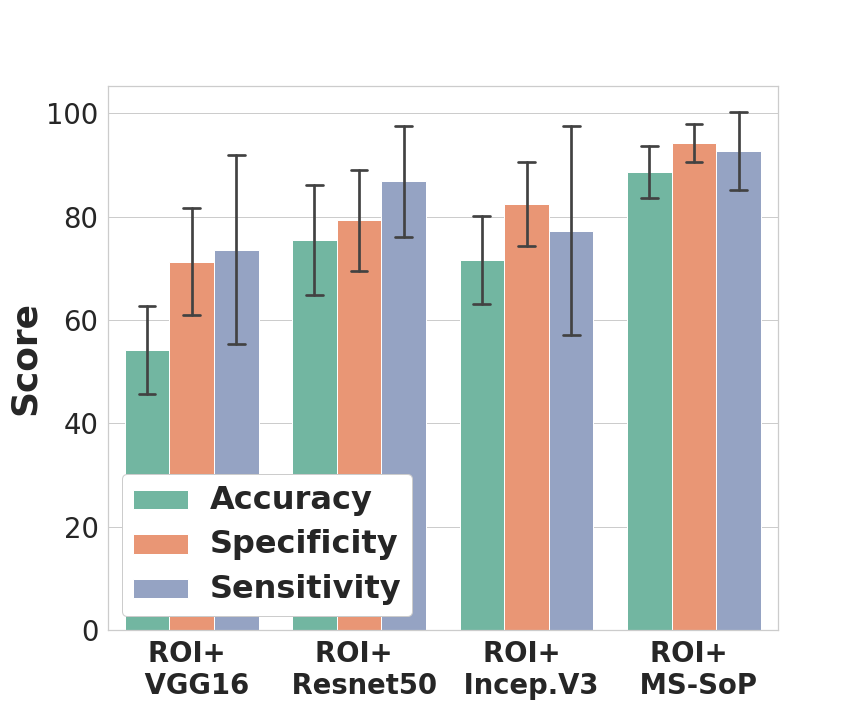
\includegraphics[width=\linewidth]{figs/gbcnet/roi_models.png}
    \caption{}
    \label{fig:perf_attn_models}
    \end{subfigure}
	\begin{subfigure}[b]{0.23\linewidth}
		\centering
		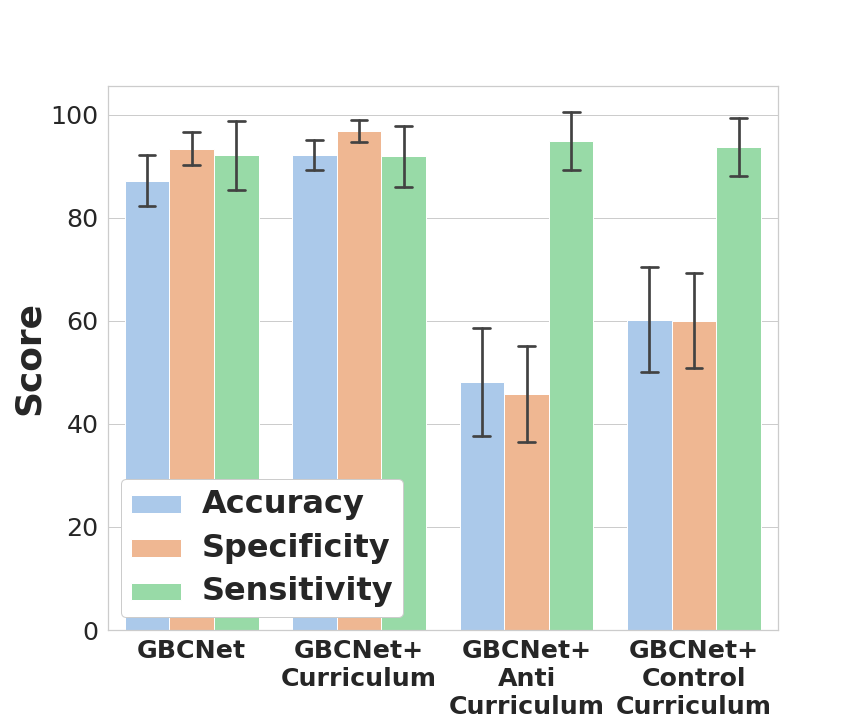
\includegraphics[width=\linewidth]{figs/gbcnet/curr_pred.png}
		\caption{}
		\label{fig:ablation1}
	\end{subfigure}
	%
	\begin{subfigure}[b]{0.23\linewidth}
		\centering
		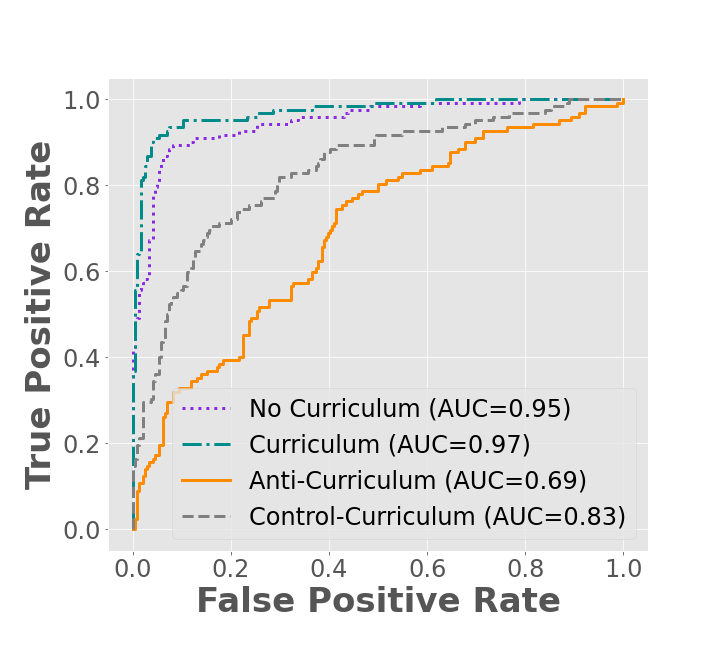
\includegraphics[width=\linewidth]{figs/gbcnet/roc.png}
		\caption{}
		\label{fig:ablation2}
	\end{subfigure}
		\begin{subfigure}[b]{0.23\linewidth}
		\centering
		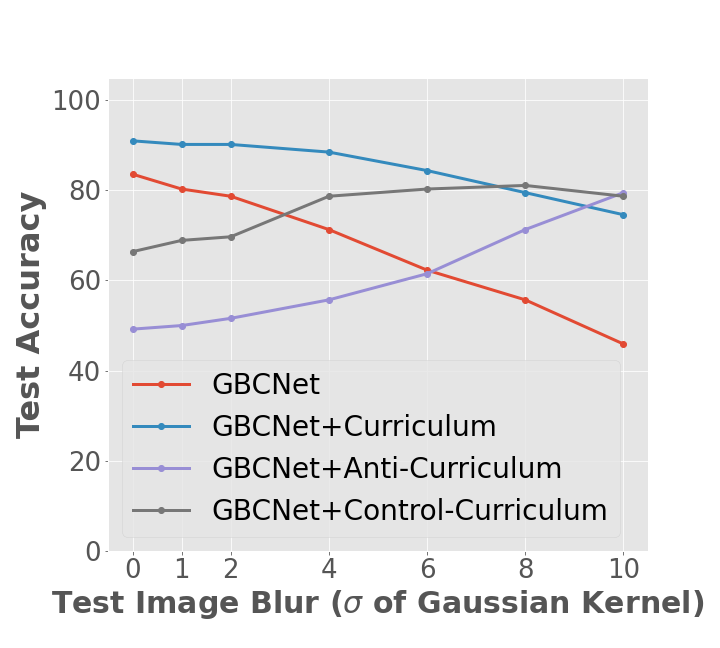
\includegraphics[width=\linewidth]{figs/gbcnet/acc-mr.png}
		\caption{}
		\label{fig:ablation3}
	\end{subfigure}
	\caption[Ablation study]{Ablation study. (a) Comparison of accuracy, specificity, and sensitivity for applying different classification networks (VGG16, ResNet50, Inception-V3, and MS-SoP) on the localized \gb. We have reported the 10-fold cross validation results. (b) The efficacy of the proposed training regime in terms of accuracy, specificity, sensitivity. (c) ROC-AUC for different training regimes on the test set. (d) The proposed curriculum generalizes better at different resolutions. }
	\label{fig:diff_images}
\end{figure}

\subsection{Ablation Study}
%
\myfirstpara{Choice of Classifier in GBCNet}
%
We have plugged in other deep classification networks in place of the proposed MS-SoP classifier in the GBCNet framework. \cref{fig:perf_attn_models} summarizes the results. The MS-SoP classifier on GBCNet provides the best \gbc detection accuracy. Using the classifiers on the \rois improves the sensitivity and accuracy for ResNet50 and VGG16. However, the drop in specificity results in performance degradation for Inception-V3 as the sensitivity was not improved.  

\mypara{Choice of Training Regime}
%
We used the proposed GBCNet model to assess the influence of the visual acuity-based curriculum. We compare the curriculum with two possible alternatives - (i) \emph{anti-curriculum} that initially trains with high resolution and progressively lowers the resolution, and (ii) \emph{control-curriculum} where the samples are not sorted resolution-wise, and the curriculum contains a random set of blurred samples. Note that the control-curriculum can also be thought of using Gaussian blurring as a data augmentation where the probability of choosing a particular $\sigma$ is equal to the fraction of epochs the $\sigma$ used during the curriculum. \cref{fig:ablation1} and \ref{fig:ablation2} show the performance of the various curriculum strategies on the performance on GBCNet.  %\cref{fig:gbc_curr_blur} shows the ROC with the AUC for GBCNet with different curriculum. 
%Additionally, \cref{tbl:curr_texture} shows the performance improvement of attention region-based classifiers when trained with the proposed curriculum.
Further, to understand how various curriculum strategies affect a model's generalization at different resolutions, we blur the test set using different values of $\sigma$ and evaluate the models on these images (\cref{fig:ablation3}). 
%The results of this comparison can be seen in \cref{fig:ablation3}. 
We see that the model trained using the proposed curriculum generalizes well across different image resolutions, which is an indicator of better spatial understanding.

\begin{table}[t]
	\centering
	\footnotesize
%	\captionsetup{width=\linewidth}
%    \setlength{\tabcolsep}{6pt}
%	\resizebox{\linewidth}{!}{%
    \begin{tabular}{@{}lccc@{}}
    \toprule[1pt]
    \textbf{Model} & \textbf{Spec.} & \textbf{Sens.} \\
    \midrule[0.5pt]
    ROI+MS-SoP (GBCNet) & 0.942 $\pm$ 0.037 & 0.923 $\pm$ 0.071 \\
    ROI+MS-SoP (channel-wise pooling) & 0.904 $\pm$ 0.047 & 0.861 $\pm$ 0.068  \\
    ROI+MS-SoP (spatial pooling) & 0.900 $\pm$ 0.064 & 0.882 $\pm$ 0.064 \\
    ROI+MS (w/o SoP) & 0.887 $\pm$ 0.060 & 0.872 $\pm$ 0.064 \\
    ROI+SoP (w/o MS) & 0.914 $\pm$ 0.048 & 0.854 $\pm$ 0.079 \\
    \bottomrule[1pt]
    \end{tabular}
%	}
	\caption[Ablation of the proposed MS-SoP network]{Ablation of Ms-SoP. We show the specificity and sensitivity of MS-SoP with two alternatives - MS-SoP with (i) only channel-wise and (ii) only spatial pooling. We also show the efficacy of using multi-scale and second-order pooling in conjunction.}
\label{tbl:ms-sop-ablation}
\end{table}

\mypara{Components of the MS-SoP Classifier}
%
We present the ablation study on the MS-SoP classifier in \cref{tbl:ms-sop-ablation}. We show the effect of the multi-scale and second-order pooling components on the specificity and sensitivity of the model. We also show the relevance of the channel-wise and spatial pooling in the second-order pooling.